%%%%%%%%%%%%%%%%%%%%%%%%%%%%%%%%%%%%%%%%%%%%%%%%%%%%%%%%%%%%%%%%%%%%
\section{Organization}
\label{sec:fdsp-pd-org}
%\metainfo{\color{red}\bf  Content: Segreto/Warner/Mualem}
%\metainfo{(Length: TDR=20 pages, TP=4 pages)}

%%%%%%%%%%%%%%%%%%%%%%%%%%%%%%%%%%%
\subsection{Single-Phase Photon Detection System Consortium Organization}
\label{sec:fdsp-pd-org-consortium}
%\metainfo{\color{blue} Content: Segreto}


The PDS consortium follows the typical organizational structure of DUNE Consortia:
\begin{itemize}
\item A Consortium Lead (Ettore Segreto) provides overall leadership for the effort, and attends meetings of the Executive and Technical Boards.
\item A Technical Lead (David Warner) provides technical support to the consortium lead, attends the Technical Board and Integration/Project meetings, oversees the project schedule and WBS, and oversees the operation of the project working groups.  In the case of the PDS, the Technical Lead is supported by a Deputy Technical Lead (Leon Mualem).
\end{itemize}

\begin{dunefigure}[PD Consortium organization chart.]{fig:pds-org.pdf}
{PD Consortium organization chart.}
 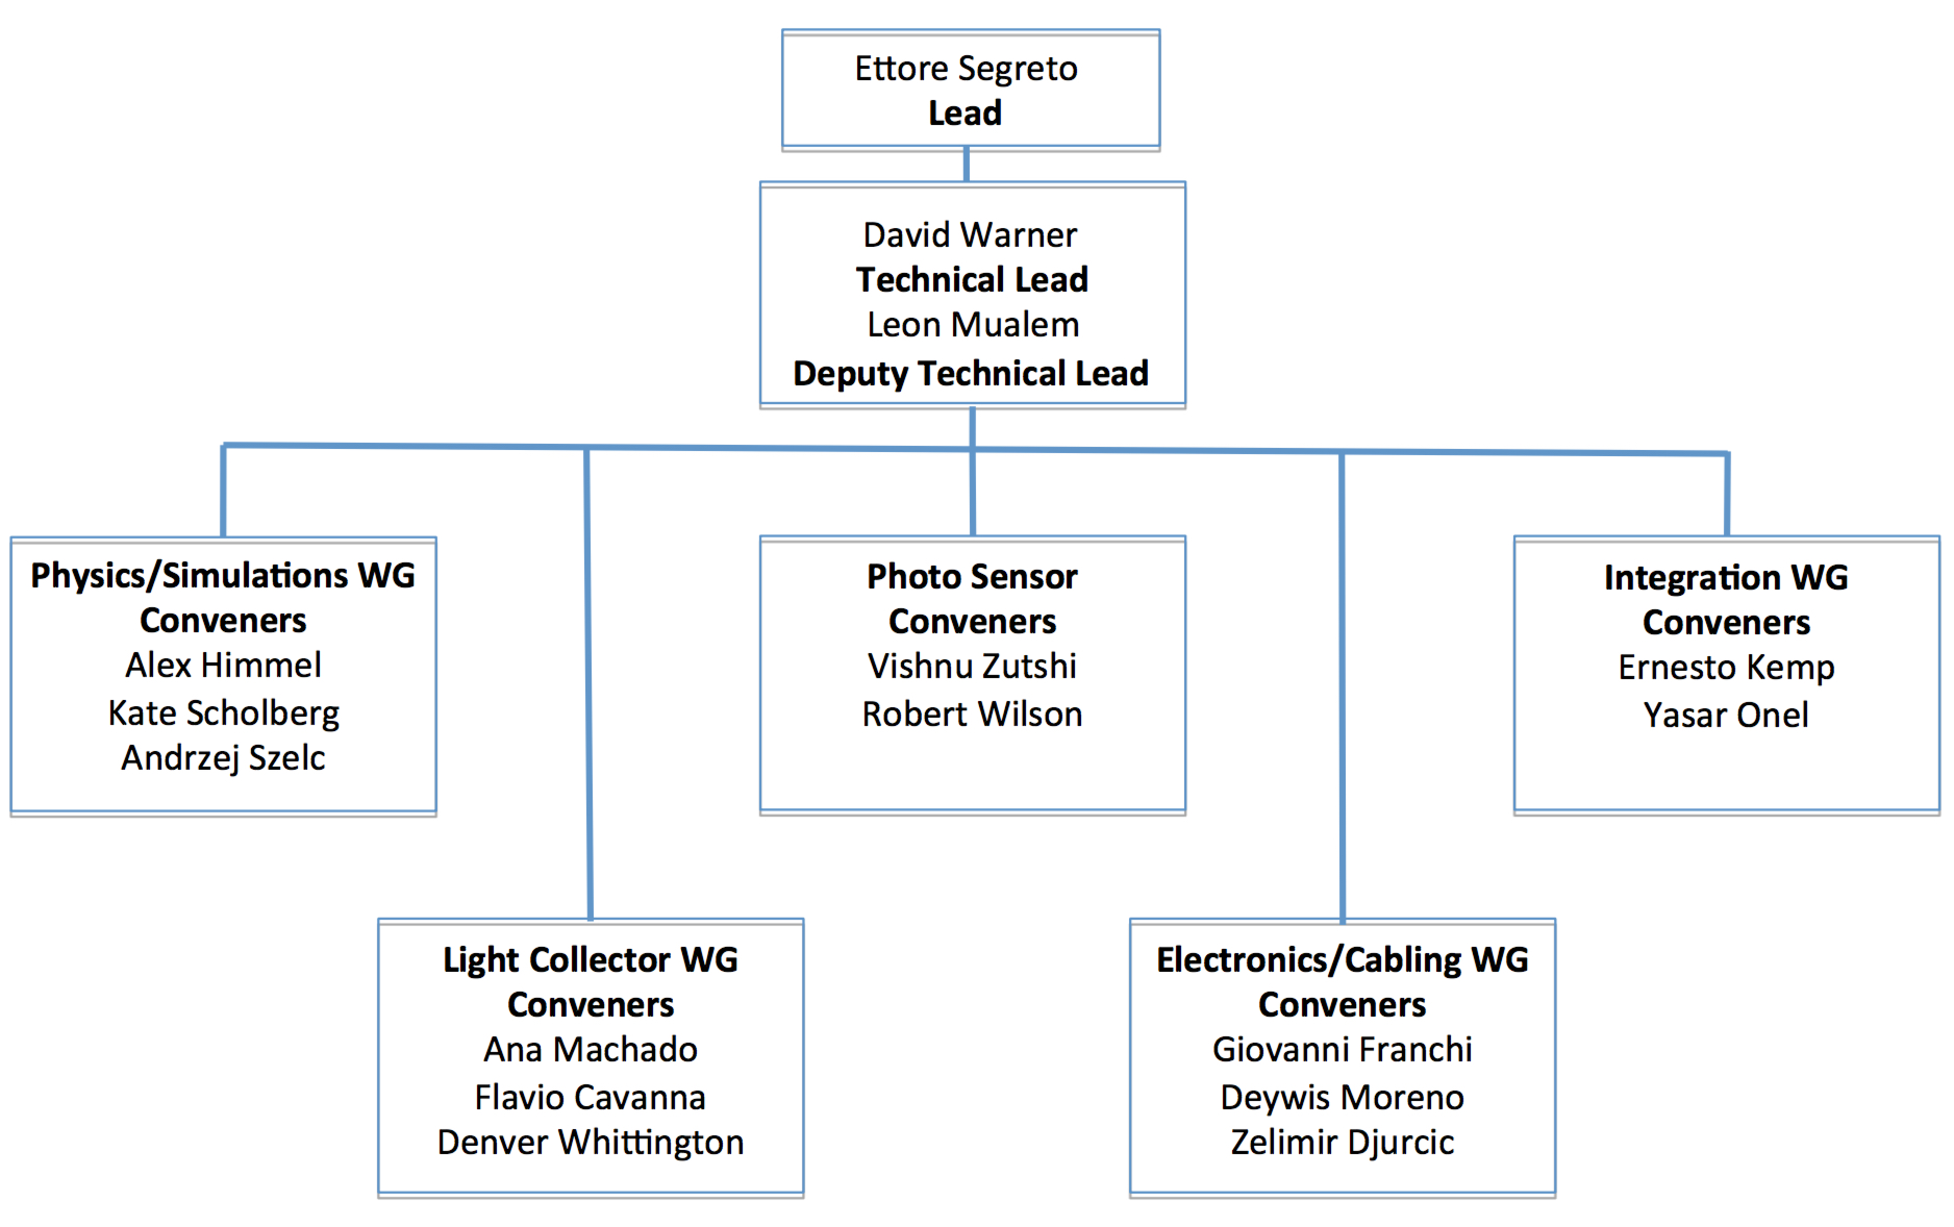
\includegraphics[width=0.8\columnwidth]{pds-org.pdf}
\end{dunefigure}

Below the leadership, the consortium is divided up into five working groups, each led by two or three working group conveners as shown in the PDS Management Table of Organization.  Each working group is charged with one primary area of responsibility within the consortium, and the conveners report directly to the technical lead regarding those responsibilities.  As the consortium advances to a more detailed WBS and project schedule, it is envisioned that each working group will be responsible for one section of those documents.

The Working group conveners are appointed by the PDS Project Lead and Technical Lead, and the structure may evolve as the consortium matures and additional needs are identified. 

%%%%%%%%%%%%%%%%%%%%%%%%%%%%%%%%%%
\subsection{Planning Assumptions}
\label{sec:fdsp-pd-org-assmp}
%\metainfo{\color{blue} Content: Segreto/Warner}

Plans for the PDS consortium are based on the overall schedule for DUNE that assumes that the first APAs need to be fully populated with photon detector modules and tested toward the \todo{set date}end of 20XX. The APA production needs to be completed about YY months later and the installation in the cryostat should be
finished by \todo{set date}mid-20ZZ.  This defines the time window for the completion of the final development program on the light collectors: A final down-select to a baseline light collector option, photosensors, and front-end electronics needs to be made by late-February 2019.  Due to the early stage of development for the ARAPUCA light collector system, we may maintain an alternate light collector option up to the pre-production review in September of 2020, but all other systems must be defined prior to the TDR. 

For planning purposes we assume that the photon detector system modules will undergo final assembly and testing at one or more PDS assembly facilities, with an initial 
assembly rate of approximately 20 modules per week, accelerating to 40 modules per week in the second half of module fabrication.

We further assume that the modules will be shipped from the to a detector integration facility, at a site to be determined later, to be integrated along with the cold electronics into the APA frames and cold tested in a cryogenic test facility.  We plan for an initial rate of two APAs per week, with the possibility of accelerating to four APAs per week as production lessons are learned.  PD personnel will be present at the integration facility to oversee the installation and testing.

Meeting this timeline requires that the development of the ARAPUCA system be aggressively pursued throughout CY2018, with a goal of testing near-final prototypes in the late fall of 2018 and allowing technology comparisons between the ARAPUCA and the better-developed bar technologies in winter of 2019.

Additional development efforts prior to the TDR will focus on

\begin{itemize}
\item Identifying and selecting reliable cryogenic photosensor (SiPM) candidates
\item Reducing cost and optimizing performance of front-end electronics
\item Solidifying PDS performance requirements from additional physics simulation efforts
\end{itemize}

We assume that for apart from the these items, where rapid development is still
required, most of the detector components to be delivered by the PDS consortium
will require only minor changes relative to the protoDUNE components. For this reason the modifications of these other detector components will be delayed until 2019, which will also help with the availability of funding. Exceptions will be made for further development in test stands for cabling studies, and for interface engineering required to ensure satisfactory integration of the PDS with the APA and cold electronics systems.

%%%%%%%%%%%%%%%%%%%%%%%%%%%%%%%%%%%
%\subsection{WBS and Responsibilities}
%\label{sec:fdsp-pd-org-wbs}
%\metainfo{\color{blue} Content: Warner/Mualem}

%%%%%%%%%%%%%%%%%%%%%%%%%%%%%%%%%%
\subsection{High-Level Schedule}
\label{sec:fdsp-pd-org-cs}
%\metainfo{\color{blue} Content: Warner/Mualem}

The high-level schedule for the photon detector consortium through submission of the TDR at the end of Q2 in FY19 is detailed in Figure~\ref{fig:pds-sched-to-tdr}
\begin{dunefigure}[PD consortium schedule through to the TDR.]{fig:pds-sched-to-tdr}
{Photon Detector Consortium schedule through to the TDR.}
 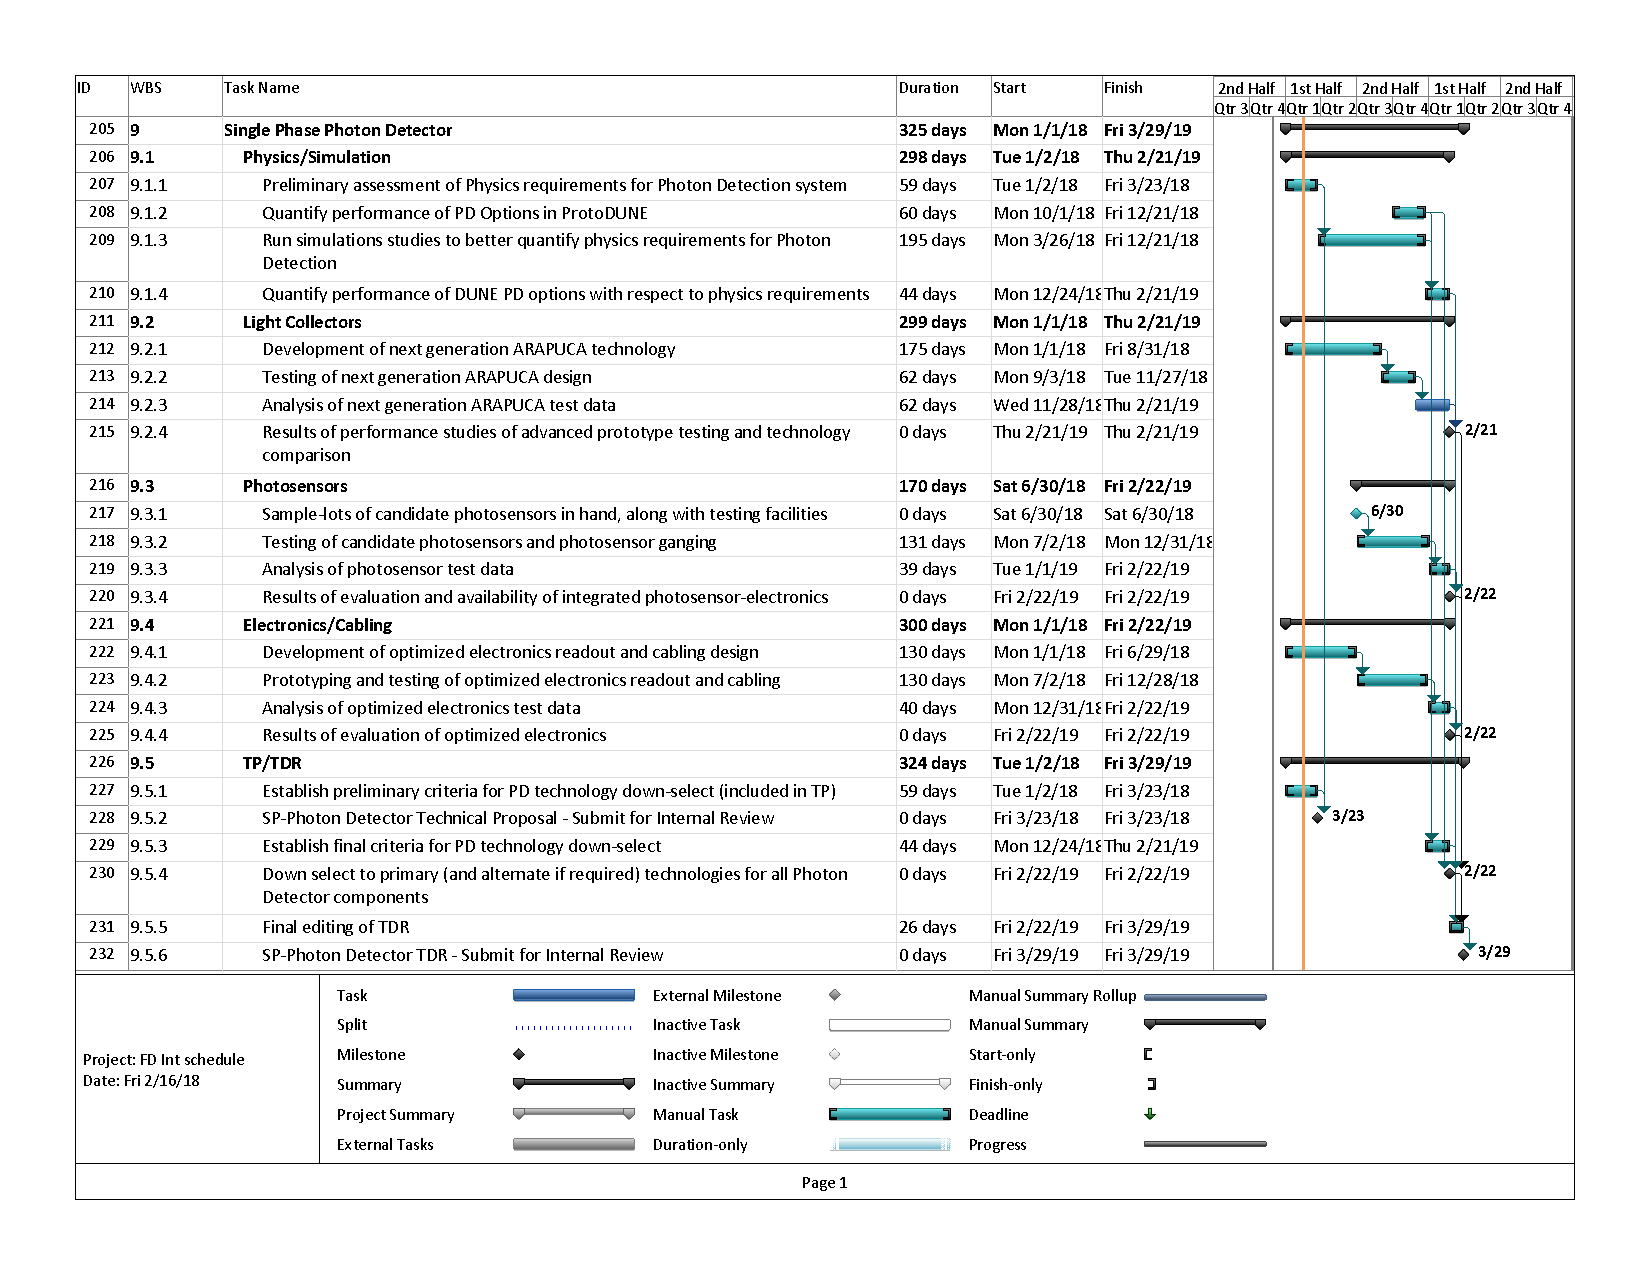
\includegraphics[width=1.0\columnwidth]{pds-sched-to-tdr.pdf}
\end{dunefigure}


Key milestones are listed in Table~\ref{fig:pds-keymilestones}.

\begin{dunetable}[Key Milestones.]
{ll}
{fig:pds-keymilestones}
{Key Milestones.}
Preliminary PD technology selection criteria determined				&3/21/18\\ \toprowrule
Results from final prototype light collector studies available			&2/21/19\\ \colhline
Final PD technology selection criteria available						&2/21/19\\ \colhline
Down-select to primary (and potential alternate) light collector technology	&2/22/19\\ \colhline
Submit initial TDR draft for internal review							&3/29/19\\ \colhline
\end{dunetable}

The Post-TDR PD schedule is still being developed, based on input from the far site detector integration team and preliminary planning in the PD group.  Some preliminary high-level milestones are listed in Table~\ref{fig:pds-posttdrkeymilestones}.

\begin{dunetable}[Preliminary Post-TDR Key Milestones.]
{ll}
{fig:pds-posttdrkeymilestones}
{Preliminary Post-TDR Key Milestones.}
PD pre-production review(s) complete					&9/2020\\ \toprowrule
Initial PD module fabrication begins						&3/2021\\ \colhline
Final PD production review based on initial production QA)		&9/2021\\ \colhline
First 25\% PD modules delivered for installation					&6/2022\\ \colhline
Installation into APAs begins							&12/2022 (?)\\ \colhline
PD fabrication complete (first 10 kt detector)				&	6/2023\\ \colhline
Installation into APAs complete (first 10 kt detector)			&	9/2023 (?)\\ \colhline
\end{dunetable}
